%!TEX root = ../Main.tex

\chapter{Vulkan API Overview/Workflow}
\label{cha:VulkanOverview}
  \todo[inline]
  {
    High level goals of this chapter:

    -- Explain important Vulkan terms.

    -- Make clear what an object is.

    -- Explain Vulkan interfaces and patterns.
  }
  \todo[inline]
  {
    The Vulkan Graphics \gls{api} workflow, object creation, patterns (vkCreate/vkDestroy, vkAllocate/vkDeallocate), synchronization.

    Listing and short explanation of Vulkan components such as buffers, images, command buffers.

    Also mention that many details are being omitted in this work/paper because it would be too much information. So make it clear this is not a comprehensive documentation of the API.

    Note that when talking about a \textit{device}, a logical device is meant. When referring to the actual hardware component the term \textit{physical device} will be used.
  }

  This chapter provides an overview of the Vulkan API and explains some concepts in greater detail. The Vulkan 1.0 specification~\cite{vkspec} was consulted for most of the information presented in this chapter. In some places, an abbreviated form is used when referring to several Vulkan commands at once, e.g. \lstinline{vkPlaceholder*} would refer to all Vulkan commands that begin with the character string \textit{vkPlaceholder}, e.g. \lstinline{vkPlaceholderCommand}. The asterisk is used as a wildcard character.

  Vulkan does not define platform specific functionality as part of the Vulkan core specification. Instead, Vulkan provides extensions to support platform specific functionality. Extensions are discussed in section~\ref{sec:LayersAndExtensions}.

  \todo[inline]{Explain the roles of \gls{application}, \gls{host}, \gls{device}. Maybe also \gls{driver}.}

  \section{Workflow and Patterns}
  \label{sec:WorkflowAndPatterns}
    The Vulkan API was designed to be consistent and explicit. Many patterns can be found in the Vulkan code style that make it easier for the \gls{application} to use the API effectively. This section is a walkthrough of the basic steps that needed to set up a Vulkan graphics pipeline to present an image to a display.

    Vulkan makes use of \textit{handle} types allowing the \gls{application} to track objects created with the API. The first object that has to be created is a Vulkan instance. The Vulkan instance can be used to query available physical \glspl{device} that provide Vulkan support. These physical \glspl{device} can be queried for certain capabilities, such as supported image formats and hardware features, to aid in deciding which physical device to use for the \gls{application}. A physical device can subsequently be used to create a logical device, or just device. The number of \glspl{device} created from a physical device is not limited. When a device is created, all queues associated with it are created as well. This is why there is no \lstinline{vkCreateQueue} but rather \lstinline{vkGetQueue} command. Among other things, \glspl{device} are used to allocate Vulkan objects or GPU memory. Changes made on Vulkan objects do not have global side-effect observable with the regular Vulkan API\todo{Elaborate. Contrast with OpenGL}. However, \glspl{driver} and Vulkan layers or extensions are free to modify their own state across Vulkan object boundaries.\todo{Redundant sentence? This should be a given.}

    \begin{figure}
      % \includegraphics{Main/Images/VulkanInitialization}
      \missingfigure{Initializing a Vulkan device and retrieving the queue to support the previous paragraph.}
      \centering
      \caption{}
      \label{fig:VulkanInitialization}
    \end{figure}

    \todo[inline]{Describe/mention GPU queues in the introduction chapter.}

    Once a device handle has been acquired, the \gls{application} can create a swapchain to establish a connection between a specific queue on the device and a platform specific presentation engine. A swapchain contains a number of \textit{presentation images}. Usually, these images are used to store the results of the graphics pipelines. At the time these images are presented, they have to be in a special layout reserved for presentation purposes.

    In order to produce images for the presentation engine to consume via the swapchain, a graphics pipeline needs to be created. This graphics pipeline consists of one or more render pass objects that hold information about how to complete a rendering step. \todo{Rewrite this sentence? Seems wonky.}Examples of the render pass state that has to be set are the used pipeline stages, such as vertex or fragment shader stages or compute shader stages, as well as setting framebuffer attachments. Render passes can be organized into subpasses which can be set up to depend on other subpasses, e.g. for post-processing.

    With a graphics pipeline in place, command buffers can be used to record rendering commands such as copying \gls{device} memory to another location or issuing drawing commands. In order to record commands, the command buffer needs to be set into recording mode. For more information about command buffers, refer to chapter~\ref{cha:GpuResources}.

    Vulkan objects can be created using \lstinline{vkCreate*} commands with the help of \lstinline{Vk*CreateInfo} structures. These info structures contain parameters to create the requested type of object. The contents of such info structures are specific to each creation command and require the \gls{application} developer to consult the Vulkan specification in order to provide correct input data. All \lstinline{vkCreate*} commands return handles to the objects they create. When the object is no longer in use, these handles can be used to destroy the object with the help of \lstinline{vkDestroy*} commands. For every \lstinline{vkCreate*} command Vulkan provides a corresponding \lstinline{vkDestroy*} command. The commands \lstinline{vkCreateBuffer} and \lstinline{vkDestroyBuffer} are examples for this.

    \todo{Explain memory pools briefly.}When Vulkan objects are allocated from memory pools, or directly from \gls{device} memory, calls to \lstinline{vkAllocate*} commands have to be made. These commands are accompanied by \lstinline{vkFree*} commands that return resources to their origin where they originally were acquired from. The general rule is that all objects allocated from pools are released as soon as the pool itself is released. Using Vulkan objects that are released results in undefined behavior, similar to using freed memory in \gls{ccpp}.

    Unlike other APIs, Vulkan does not do any object tracking or reference counting to manage object life times. It is the responsibility of the \gls{application} to destroy or free Vulkan objects at the appropriate times, i.e. when they are no longer in use and will not be used in the future by either the \gls{host} or the device.

    Vulkan objects are not designed to be thread-safe. This means that accessing or modifying a Vulkan object from more than one thread at once can lead to race conditions or other undesirable behavior. It is the responsibility of the \gls{application} to employ proper synchronization mechanisms on the \gls{host} to ensure Vulkan objects are never \todo{Clarify that it's read and write access. Maybe also explain why?}accessed concurrently.

  \section{Layers and Extensions}
  \label{sec:LayersAndExtensions}
    \todo[inline]{Layers are instance-only, extensions are both on the instance-level as well as the device-level.}

    Vulkan is designed to be extensible by thirdparty \glspl{application}. The two mechanisms provided are called layers and extensions.

    A layer in Vulkan can be thought of as an observer to the API calls done by the \gls{application}. It does not add new types or commands the \gls{application} can use directly.\todo{Elaborate more to make it crystal clear. Make sure to mention no layers are required to be active for Vulkan to work properly.}

    \begin{figure}
      \centering
      % \includegraphics{Main/Images/VulkanLayers}
      \missingfigure{Illustration of Vulkan with some layers between it and the application.}
      \caption{Illustration of the presentation engine being connected to a device using a swapchain.}
      \label{fig:VulkanLayers}
    \end{figure}

    The \todo{Reference}LunarG SDK, for example, comes with a set of layers to validate usage of the Vulkan API. This is extremely useful during development as it allows the \gls{application} to focus on their code rather than the perfect use of the Vulkan API. It should also be noted that bare Vulkan, without any validation layers enabled, does not do any error checking. When the \gls{application} passes an invalid combination of flags to some Vulkan function, it is undefined behavior and has to be corrected by the \gls{application}.

    \todo[inline]{Maybe rephrase the paragraphs above by first explaining the concepts and then giving examples in a separate paragraphs.}

    As opposed to layers, extensions are able to provide new or add to existing functionality. The motivation for extensions is to keep the Vulkan core functionality small and provide specific functionality via such extensions. In fact, the Khronos Group provides built-in extensions for both common and platform specific functionality.

    \begin{figure}
      \centering
      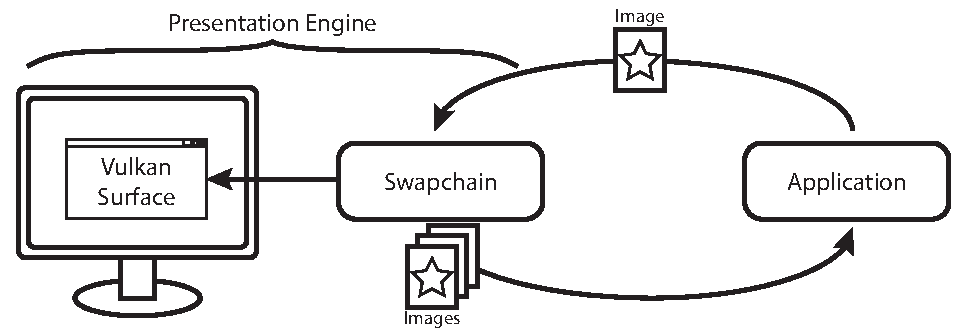
\includegraphics{Main/Images/PresentationEngine}
      \caption{Illustration of the presentation engine being connected to a device using a swapchain.}
      \label{fig:PresentationEngine}
    \end{figure}

    The most important extensions are arguably the swapchain and platform specific surface extensions. These extensions enable the \gls{application} to create a Vulkan swapchain and a compatible surface object that is used by the presentation engine to present an image. \todo{Only when they want to see something! duh.}Vulkan requires the \gls{application} to create a platform specific window which is then used when creating a Vulkan surface. This surface is subsequently used to create the swapchain that acts as the connection between a device and the surface. With this constellation, the presentation engine is able to properly present an image on a platform specific window. The extension to create a swapchain is called \todo{Explain KHR within this string. Maybe do this somewhere early in this chapter?}\lstinline{VK_KHR_swapchain}. It adds several types and commands to create and interact with a swapchain. The concept of a swapchain is independent of the platform but it requires the help of platform specific functionality in order to work. On Windows platforms, for example, the \gls{application} needs to enable the \lstinline{VK_KHR_win32_surface} extension in order to link a swapchain to a Win32 window. From the perspective of the \gls{application}, there is no need to care about distinguishing between platforms when creating a swapchain but they do have to when creating and connecting the swapchain to a platform specific surface.

    \todo[inline]{Restructure the paragraphs below more logically.}

    Extensions can be loaded and enabled on both instance-level and device-level. Instance-level extensions provide functionality that is generally independent of the hardware.

    The extension \lstinline{VK_EXT_debug_report}, for example, is an instance-level extension. It enables the \gls{application} to provide a callback function that is used by Vulkan layers or extensions to communicate with the \gls{application}. If validation layers are enabled, this is how they would tell the \gls{application} about any validation concerns or violations. An example for a device-level extension is the aforementioned \lstinline{VK_KHR_swapchain} extension. Not all physical \glspl{device} have to be capable of rendering graphics images. In the end it is up the extension author on which level they provide their extension.

  \section{Resources and Memory Allocation}
  \label{sec:MemoryManagement}
    Memory in Vulkan is categorized in either \gls{host} memory or \gls{device} memory.

    Host memory is used by the \gls{driver} for data that is not visible to the device. The \gls{application} has the option to supply memory allocators to the \gls{driver} to control how \gls{host} memory is allocated. Host memory allocations are not \todo{conducted => made?}conducted in performance critical code paths. In general, supplying custom memory allocators may not significantly affect efficiency of the \gls{application}. Instead, it is an opportunity for \glspl{host} on embedded systems to control memory allocations or for informational purposes such as logging memory allocations done by the \gls{driver}.

    The physical storage of a device is called device memory. Device memory is separated into different types of heaps. Each of these heaps has a defined size and a combination of flags. The flags indicate whether memory from that heap is visible to the \gls{host}, for example, or whether the memory is completely local to the device. In order for the allocated memory to be useful, the \gls{application} has to bind it to a resource.

    There are two fundamental types of resources in Vulkan, the buffer resource and the image resource.

    \begin{description}
      \item[Buffers]
        A buffer is treated as a one-dimensional, unformatted, contiguous block of memory that can be used by the \gls{application} to upload general purpose data to the device. This data may then be used during shader execution, for example, or may be copied and transformed on the GPU to another buffer or even an image.

      \item[Images]
        As opposed to buffer resources, an image contains more information about how the underlying memory is used. For example, an image has a particular format, such as having red-green-blue channels, each channel using 8 bits of memory. An image may also be in a particular layout, e.g. in \textit{shader read-only} layout which is required when the image is supposed to be used by a shader. Another important image property is the image tiling. An image may either exist in linear tiling or optimal tiling. Linear tiling means that the underlying data of the image is layed out in memory in a linear fashion. The data will be in the same memory layout as it was when it was uploaded. The memory layout of the image data in optimal tiling, however, is not specified by Vulkan. The \gls{driver} is free to lay out the data in memory as it sees fit. This is done in order to improve performance. Parts of the actual physical device may process an image faster in certain circumstances when the image data is not layed out linearly in memory.
    \end{description}

    \todo[inline]{Describe buffer views and image views.}

  \section{Command Buffers}
  \label{sec:CommandBuffers}
    Vulkan provides a number of commands that can be executed on the GPU. These commands are recorded into command buffers. Command buffers are allocated from command pools.

    Command buffers have some externally visible state and some internally managed state that is unqiue to this command buffer and never shared with other command buffers. The externally visible state defines which operations are currently valid on a given command buffer.

    \todo{Briefly explain initial, record, and execute states.}In the \textit{initial} state, the internally managed state of the command buffer is undefined. From the \textit{initial} state, a command buffer can be brought into the \textit{recording} state. In this state the command buffer accepts commands to be recorded to the internally managed state. Once recording of all commands is done, the command buffer can be brought to the \textit{executable} state. In this state, the command buffer may be submitted to a queue which will execute the recorded commands on the GPU. Without implicit dependencies or explicit synchronization, \todo{Check the spec for whether this is actually true!}the order in which commands are executed on the GPU is not defined. This means that submitted commands may run concurrently or in a different order than they were recorded in.

    The internal state of a command buffer is not reset when submitting it to the queue. This enables the \gls{application} to record a command buffer once and submit it several times.

    The \gls{application} may utilize several threads of execution to allocate command buffers from a command pool. If all threads used the same command pool or command buffer, they would need to synchronize access to that pool, as per the Vulkan specification. However, creating a command pool for each thread eliminates the need for synchronizing command buffer allocation. This can be leveraged to achieve maximum performance by dispatching work on several threads, where each is allocating command buffers at will filling them with data to be submitted to the queue later on the main thread.

  \section{Pipelines}
    \todo[inline]
    {
      Describe descriptor-sets, descriptor-pools, etc?

      Also describe uniform buffers and render targets in framebuffer?

      Shader stages in general should have been described in chapter 1.
    }

    \begin{figure}
      \centering
      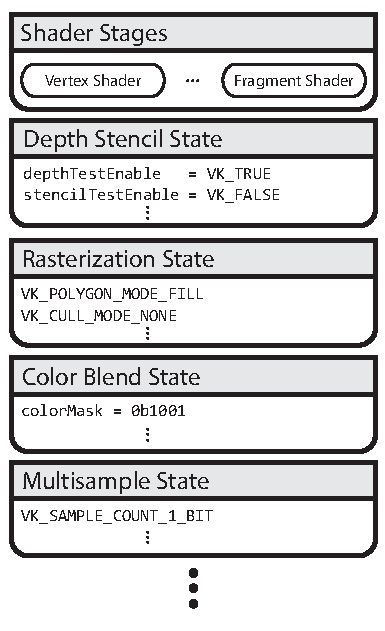
\includegraphics{Main/Images/GraphicsPipeline}
      \caption{Graphics pipeline setup.}
      \label{fig:GraphicsPipeline}
    \end{figure}

    Vulkan uses the concept of pipelines to describe how work is performed on the GPU. It supports compute and graphics pipelines. The compute pipeline consists only of a single programmable stage. The graphics pipeline, however, is considerably more complex. It has multiple fixed function stages and five programmable stages, called shader stages. Some of the fixed-function stages have a configurable state that can be manipulated by the \gls{application}. For example, the rasterization stage can be configured to interpret incoming vertex data as either a list of points, lines, or filled polygons with more than two sides.

    Programs that are designed for use in shader stages are called shaders. Shaders are supplied to Vulkan in \gls{spirv} format. \gls{spirv} is a high-level graphics and parallel compute programming language provided in \todo{Mention need to convert from GLSL or others to SPIR-V}binary form. The specification of \gls{spirv} is entirely maintained by the the Khronos Group \cite{spirvspecprov}. The five shader stages are listed below.

    \begin{itemize}
      \item Vertex shader stage
      \item Tesselation control shader stage
      \item Tesselation evaluation shader stage
      \item Geometry shader stage
      \item Fragment shader stage
    \end{itemize}

    When defining a graphics pipeline, Vulkan requires the \gls{application} to at least specify a vertex shader. All other graphics stages are optional. Vulkan has restrictions on the possible combinations of active shader stages. Details can be found in the Vulkan specification \cite{vkspec}\todo{Remove these two sentences?}.

    \todo[inline]{Describe why having only a vertex shader stage can be useful?}

    \subsection{Pipeline Cache}
    \label{subsec:PipelineCache}

      \todo[inline]{Describe driver syncing the pipeline cache. Ref to GDC talk if it's not in the vkspec?}

      \begin{figure}
        \centering
        % \includegraphics{Main/Images/PipelineCache}
        \missingfigure{Illustration of how an \gls{application} creates a bunch of pipelines using a pipeline cache, saves that cache to disk, terminates, and loads that cache the next time the \gls{application} is started again, feeding that cache to Vulkan in order to create pipelines from it.}
        \caption{Example of an \gls{application} using the pipeline cache.}
        \label{fig:PipelineCache}
      \end{figure}

      Creating pipeline objects is a fairly heavyweight operation. To speed up pipeline creation, Vulkan provides what is called a pipeline cache. When creating a pipeline, such a pipeline cache object can be supplied by the \gls{application}. Vulkan will try to find a matching pipeline in the cache. If it finds a matching pipeline, it is loaded from the cache instead of creating a new one. If no such pipeline is found in the pipeline cache, a new pipeline is created and written to the pipeline cache. Vulkan provides a command to retrieve the serialized pipeline cache, which can be saved by the \gls{application} in whatever location is most convenient to it. This serialized pipeline cache can then be fed back to Vulkan at a later time. See figure~\ref{fig:PipelineCache} for an illustration of this process.

  \section{Synchronization}
    \todo[inline]{Maybe reduce the use of `Vulkan was designed to' throughout the document?}
    Vulkan was designed to run concurrently. Synchronization is mainly the responsibility of the \gls{application}. In order to do so, Vulkan provides four types of synchronization primitives: fences, semaphores, events, and barriers. These synchronization primitives can be used to insert execution and memory dependencies in various circumstances.

    \todo[inline]{Make it clear that these synchronization primitives are for the GPU \textbf{only}. The host may blockingly wait on queue operations to finish, though. (vkWaitForQueue, vkWaitForDevice, vkWaitForFences, vkWaitForEvents)}

    \subsection{Fences}
    \label{sub:Fences}
      A fence is a synchronization primitive used to determine the execution status of submitted operations executed on a queue. Such a fence can only be in one of two states: not signaled and signaled. The status of a fence is visible to the \gls{host}. The device itself does not use the status of a fence directly.

      In practice, a fence is most commonly used with the \lstinline{vkQueueSubmit} command, which is used to submit work to a device queue that were previously recorded to command buffers. The \gls{application} can query the fence for its status using \lstinline{vkFenceGetStatus} which determines whether the fence was signaled or not. Waiting for a fence to be signaled essentially means waiting for all of the submitted work on the queue to be finished.\todo{Make clear it's only the work that was given in the same queue submission as the fence}{} In order to wait for a fence to be signaled in a blocking\todo{Sugarcoat the term `blocking' a bit?}{} fashion the \lstinline{vkWaitForFences} command is used.

    \subsection{Semaphores}
    \label{sub:Semaphores}
      A semaphore is similar to a fence, as discussed above in~\ref{sub:Fences}\todo{Should I omit this?}, except that its status is only visible to the device. It can be used to synchronize operations within the same and between different device queues.

      The most common use case for Vulkan semaphores in a graphics \gls{application} is when presenting swapchain images to the presentation engine. First, the commands to create the final image have to be recorded to a command buffer. This command buffer then needs to be submitted to a queue in order to be executed. When submitting to the queue, a semaphore can be provided that will be signaled once the queue has finished executing all submitted commands. The same semaphore can be used when issuing the swapchain presentation command. When everything is set up like this, the presentation engine will effectively wait for the commands to produce the final image and then present it as fast as possible.

      Note that a fence can be used to achieve the same results except that it would require the \gls{host} to actively wait for the queue to finish executing, stalling any other CPU operations that could have been executed in that time. Using the semaphore in this case will result in better performance.

    \subsection{Events}
    \label{sub:Events}
      \todo[inline]{Investigate: Event host-callbacks? Or does the host need to poll?}

      Events are used to synchronize from \gls{host} to device or from device to device in a bidirectional manner. Like semaphores and fences, events are either in a signaled or in a not-signaled state. Events are inserted into command buffers in order to allow the device to signal them. This allows for more fine-grained synchronization between commands and to signal command completion to the \gls{host}. Unlike a fence, an event can be inserted at any point in the command buffer stream and thus can be used to query for synchronization without requiring that all commands in the submitted command buffer have completed execution.

      Events work in a way that can be taken advantage of when faced with a scenario that requires the \gls{application} to transform a large number of resources in batches. Given an arbitrary number of images in an \gls{application} that need to be transformed in some way that is expensive to compute, these transformations could be issued into a single command buffer, inserting a completion event between these commands. After submitting this command buffer to the queue, the \gls{application} can periodically query for completion of the individual transformation commands without the need to wait for the entire submission to finish by using fences or semaphores.

      It must be noted that events are only allowed to be insterted into command buffers that are all submitted to the same queue. This makes them unsuitable for cross-queue synchronization when such is requried.

    \subsection{Barriers}
    \label{sub:Barriers}
      \todo[inline]{Restructure paragraphs. Maybe use \textit{description} environment.}
      Barriers are used exclusively with commands recorded to command buffers. There are two kinds of barriers in Vulkan. The first kind is called an execution barrier which are used to create explicit dependencies on the completion of specific commands. The second kind is called a memory barrier which are used to depend on memory to be present in a specific form. Both kinds of barriers are combined in Vulkan as a pipeline barrier.

      \begin{figure}
        \centering
        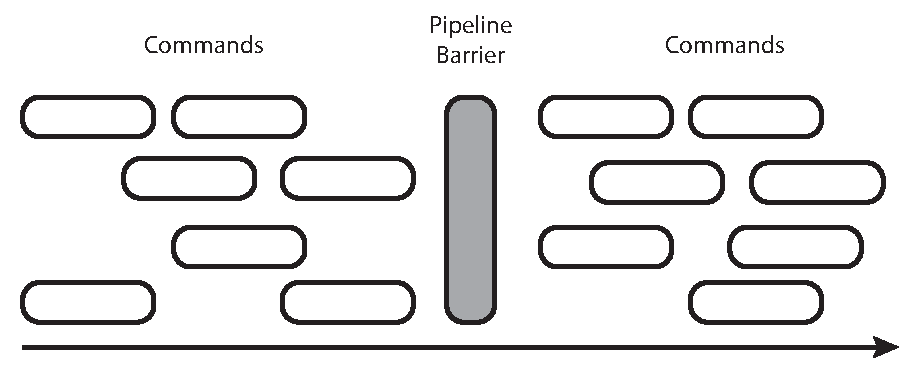
\includegraphics{Main/Images/PipelineBarrier}
        \caption{Illustration of a pipeline barrier insterted between commands in a command buffer.}
        \label{fig:PipelineBarrier}
      \end{figure}

      By inserting a memory dependency, Vulkan guarantees that all memory operations on a specified resource or memory regionto be finished once the inserted barrier has been reached. Otherwise all following commands are not able to begin executing. Analogously, an execution dependency requires all previous commands to have finished execution before starting to execute other commands inserted after the barrier.

      There are three types of memory barriers in Vulkan: Global memory barriers, buffer memory barriers, and image memory barriers.

      \subsubsection{Global Memory Barriers}
        Global memory barriers introduce a dependency to all memory objects that exist at the time of execution of the barrier. All prior memory access operations, whether they are read or write operations, must have finished before the barrier finishes execution.

        Such heavyweight memory dependencies are not needed if the memory in use is entirely cache coherent. In other words, if the rest of the system ensures that all caches are flushed at appropriate times, memory accesses from other parts of the system will be consistent and up-to-date\todo{Double-Triple-Check whether this is actually correct.}.

      \subsubsection{Buffer Memory Barriers}
        Buffer memory barriers introduce a memory access dependency on a specific region of memory associated with a buffer object. That region may encompass the entire buffer and is specified in terms of an offset, relative to the beginning of the buffer, and a size value.

        This kind of barrier can be used to transfer ownership of a buffer region to another queue family or to change access flags of that region. Transferring ownership of that buffer region to another queue family is only possible if this kind of operation has been enabled for that buffer at the time it was created. Access flags are used to control how the buffer region is accessed. They could be used to make the memory region read-only, for example, or enable \gls{host} access for it.

      \subsubsection{Image Memory Barriers}
        Image memory barriers are similar to buffer memory barriers. They can be used to transfer ownership image regions to another queue family, modify access flags, and to change the image layout. An image region is specified differently from a buffer region because of the fact that images need not be stored linearly in \gls{device} memory\todo{Refer to wherever image tiling is explained}.

        Transferring ownership of an image region is only possible if the image was set up accordingly at creation time. Modifying access flags has the same effect as with modifying access flags on a buffer region.

        Changing the layout of the image is an important operation on Vulkan images. For example, it is required for swapchain images in order to be presentable. The presentation engine requires swapchain images to be in a specific layout when presenting them so the \gls{application} must ensure that the image has that specific layout before attempting to issue the presentation command. Since the presentation layout is only meant for use by the presentation engine, the \gls{application} has to use another image memory barrier to change the layout into something that can be used by the \gls{host} \gls{application}.
